\documentclass[handout]{beamer}
% \documentclass[]{beamer}
    \usetheme{Boadilla}
    \usecolortheme{beaver}

% \usepackage[fleqn]{amsmath}
\usepackage[italicdiff]{physics}
\usepackage{siunitx}
\usepackage{amssymb,xparse}
	\usepackage[makeroom]{cancel} %% \cancelto{value}{expression}
\usepackage{caption}
\usepackage{subcaption}

\usepackage[backend=biber]{biblatex}
    \addbibresource{refs.bib}

\usepackage{graphicx}

\usepackage{courier}
\newcommand{\code}[1]{{\fontfamily{pcr}\selectfont #1}}

\usepackage{dutchcal}  %changes \mathcal, \mathbcal for script r (E&M)
\newcommand{\Letter}[1]{\mathcal{#1}}
\newcommand{\Lag}{\Letter{L}}
\newcommand{\Sl}{\ell} % Lowercase script l 
\newcommand{\Def}{\equiv}
\newcommand{\goesto}{\quad\Rightarrow\quad}
\newcommand{\prop}{\propto}
\newcommand{\p}{\partial}

\AtBeginSection[]{
  \begin{frame}
  \vfill
  \centering
  \begin{beamercolorbox}[sep=8pt,center,shadow=true,rounded=true]{title}
    \usebeamerfont{title}\insertsectionhead\par%
  \end{beamercolorbox}
  \vfill
  \end{frame}
}

\title[Analysis of Equations of State]{Analysis of Equations of State for Neutron Star Modeling and Simulation}
\author{Joseph Nyhan}
\date{6 May 2022}
\institute[CoHC]{College of the Holy Cross}

\begin{document}

    \maketitle

    \begin{frame}{Outline}
        \pause
        \begin{itemize}
            \item What is a neutron star? \pause
            \item What is an equation of state (EoS)? \pause How does it fit into our model of a neutron star? \pause
            \item How can we use an EoS to make macroscopic predictions about neutron stars? \pause
            \item What is the importance and role of an equation of state in a temporal simulation of a neutron star? \pause
            \item A derivation of an EoS and its predictions: \pause
            \begin{itemize}
                \item Quantum Hadrodynamics and the QHD-I parameter set
            \end{itemize}
        \end{itemize}
    \end{frame}

    \section{Introduction}

    \begin{frame}{Neutron Stars}
        \pause
        \begin{itemize}
            \item Dense core left behind after a supernovae explosion \pause
            \item Made mostly of neutrons, protons, and electrons\pause ; overall, is neutral \pause
            \item Radius: $\sim\SI{10}{km}$\pause ; Mass: $\sim\SI{1}{\odot}$. \pause
            \item Approximately the density of atomic nuclei ($\sim\SI{e17}{kg/m^3}$) \pause
            \item Core held together by intense gravitational attraction \pause
            \begin{itemize}
                \item Gravitational acceleration on Earth's Surface: $\approx \SI{10}{m/s^2}$ \pause
                \item Neutron star: $\approx \SI{e12}{m/s^2}$ \pause (escape velocity $\sim \SI{100000}{km/s} = $ \pause $c/3$)\pause
            \end{itemize}
            \item Why are they interesting? \pause \begin{itemize}
                \item Smallest, densest observed stellar objects \pause
                \item Exotic physics
            \end{itemize}
        \end{itemize}
    \end{frame}

    \begin{frame}{Equation of State (EoS)}
        What is an equation of state? \pause
        \begin{itemize}
            \item A relationship between \textit{energy density} (denoted $\epsilon$) \pause and pressure (denoted $P$) \pause \begin{itemize}
                \item $\epsilon = \epsilon (P)$\pause $~~ \Leftrightarrow ~~  P = P(\epsilon)$ \pause
            \end{itemize}
            \item Encodes the fundamental interparticle interactions within a neutron star \pause
            \item True EoS within a neutron star is unknown; \pause multitude of candidates, each based on a slightly different model and fit of empirical data \pause \begin{itemize}
                \item Models can be very complicated\pause ; often simplifications must be made to be solved practically \pause
            \end{itemize}
            \item Often a tabulated list of $P$ and $\epsilon$ values; \pause however, in simulation work, analytical fits may be required
        \end{itemize}
    \end{frame}

    % \begin{frame}{Using an Equation of State to Make Predictions}
    %     \begin{itemize}
    %         \item TOV equations \pause
    %         \item Mass rad
    %     \end{itemize}
    % \end{frame}


    \section{Using an Equation of State to Make Predictions}

    \begin{frame}{Using an EoS to Make Predictions}
        We want a way to understand the effects of an EoS on the observable properties of a star \pause
        \begin{itemize}
            \item e.g. total mass, total radius \pause
        \end{itemize}
        We create \textit{static solutions}; ``images'' of neutron star \pause
        \begin{itemize}
            \item solve the Tolman-Oppenheimer-Volkoff (TOV) equations \pause
            \item extract information about maximum max and radius allowed by the EoS
        \end{itemize}
    \end{frame}

    \begin{frame}{The Tolman-Oppenheimer-Volkoff (TOV) Equations}
        \pause Used to describe a static (time independent) spherically symmetric star. \pause Given by
        \begin{align*}
            \dv{m}{r} = 4\pi r^2 \epsilon, \quad \dv{P}{r} = -\frac{(4\pi r^3 P + m)(\epsilon + P)}{r^2 (1-2m/r)}.
        \end{align*}
        where $\epsilon$ is energy density, $P$ is pressure, and $m$ is ``mass.'' \pause Use EoS to determine $\epsilon~$\pause $=\epsilon(P)$. \pause 
        \medskip
        
        \begin{itemize}
            \item Initial conditions: \pause
            \[m(r=0) = 0, \quad P(r=0) \Def P_0 = \text{const.}\]\pause
            Each solution is uniquely defined by $P_0$, the \textit{central pressure}. \pause
            \item Outer conditions: Let $R,M$ to be the total radius and total mass of the star, respectively. \pause Defined by:
            \[P(R) = 0, \quad M = m(R).\]
        \end{itemize}
    \end{frame}

    \begin{frame}{TOV Equations: Computing a Solution}
        \begin{align*}
            \dv{m}{r} = 4\pi r^2 \epsilon, \quad \dv{P}{r} = -\frac{(4\pi r^3 P + m)(\epsilon + P)}{r^2 (1-2m/r)}.
        \end{align*} \pause
        \begin{itemize}
            \item Specify a central pressure $P(r=0) = P_0$ \pause
            \item Begin at very small $r \approx 0$; (\SI{e-8}{}) \pause
            \item Use a numerical integration technique \pause
            \begin{itemize}
                \item The Runge-Kutta 4 Algorithm \pause
                \item In practice, use Scipy \code{solve\_ivp}; faster due to optimized step size \pause
            \end{itemize}
            \item Integrate outwards until $P = 0$; use to define $R$, calculate $M$ \pause
            \item Store curves for $m(r), P(r)$, \pause use to calculate $\epsilon(r)$ \pause
            \item \textit{Note}: works well with tabulated EoSs; an interpolating function is often used
        \end{itemize}
    \end{frame}

    \begin{frame}{Static Solution: Example}
        \pause
        Use an EoS called ``SLy'' from \autocite{SLy_2004}. A realistic equation of state from an analytical fit of empirical neutron star data. \pause

        \begin{figure}[h!]
            \centering
            \begin{subfigure}{.5\textwidth}
                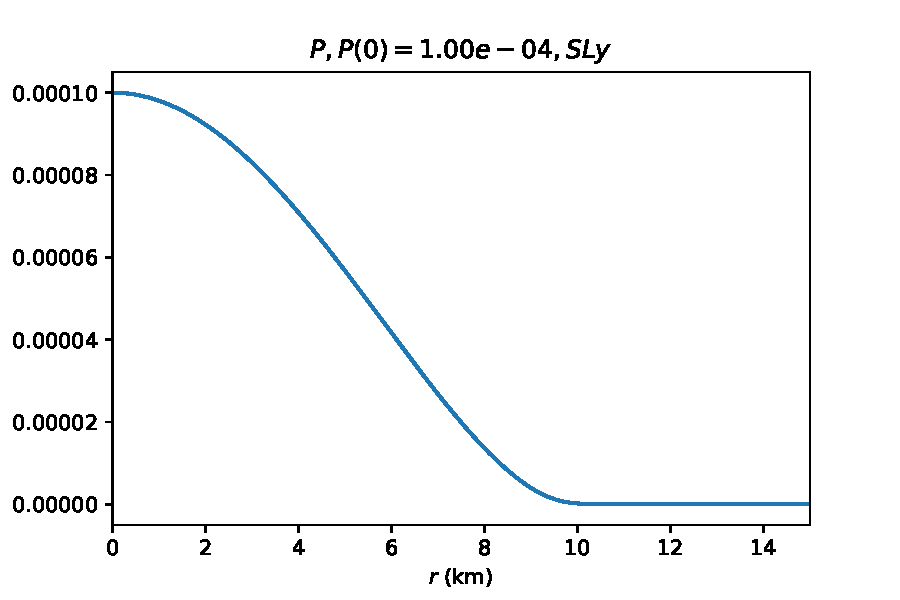
\includegraphics[width = \textwidth]{SLy_P,p0_0.0001.pdf}
            \end{subfigure}%
            \begin{subfigure}{.5\textwidth}
                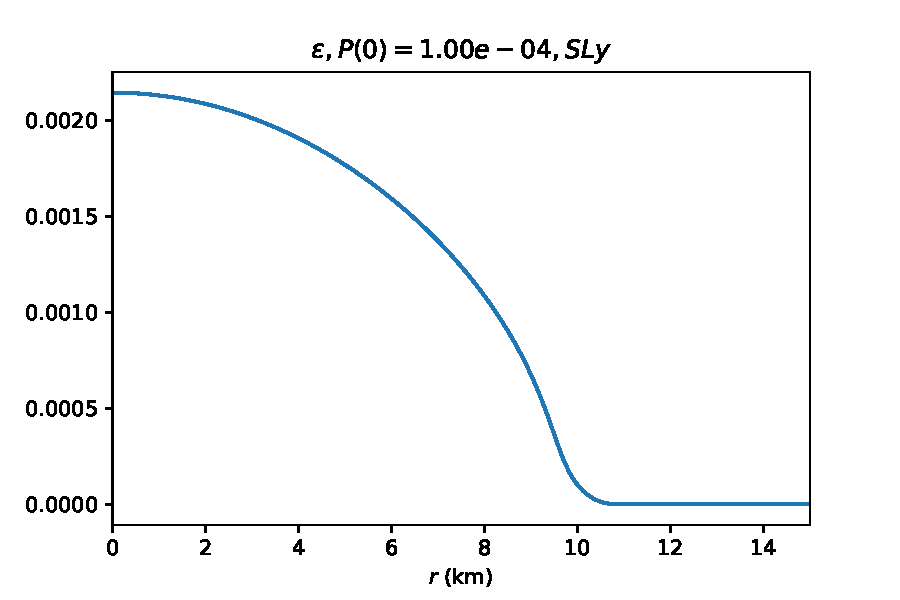
\includegraphics[width = \textwidth]{SLy_rho,p0_0.0001.pdf}
            \end{subfigure}
            \caption[]{Example static solution for $P_0 = \SI{e-4}{GeV^4}$ for an EoS called ``SLy.''}
        \end{figure}

    \end{frame}

    \begin{frame}{Static Solutions: $M(R)$ and $M(P_0)$ diagrams}
        \pause
        Single solutions don't tell much about star as a whole; instead, look at trends over lots of solutions \pause
        \begin{enumerate}
            \item Solve TOV equations for lots of $P_0$ values: \pause $P_0 \in [\SI{e-6}{}, \SI{e-1}{}](\SI{}{GeV^4}).$\pause
            \item Calculate the total mass $M$ and total radius $R$ for each value of $P_0$ \pause
            \item Plot $M(R)$ and $M(P_0)$\pause
        \end{enumerate}

        \begin{figure}[h!]
            \centering
            \begin{subfigure}{.5\textwidth}
                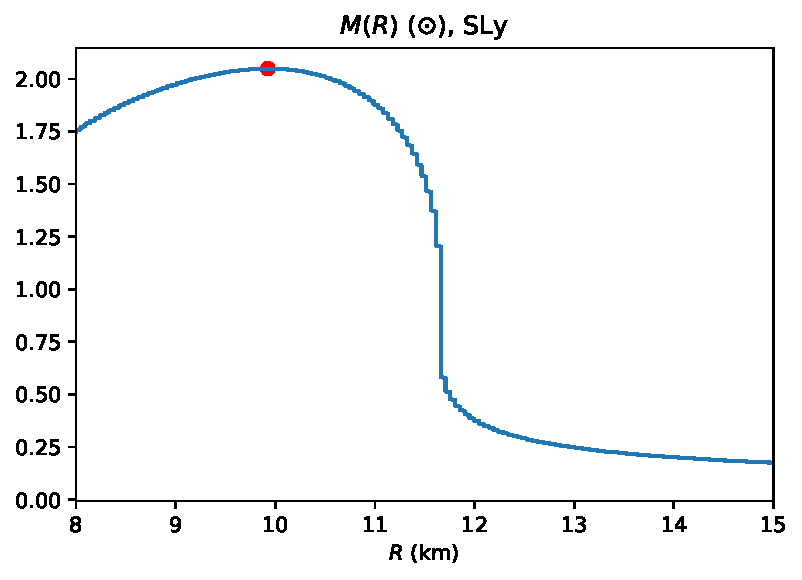
\includegraphics[width = \textwidth]{r_analysis,SLy.pdf}
            \end{subfigure}%
            \begin{subfigure}{.5\textwidth}
                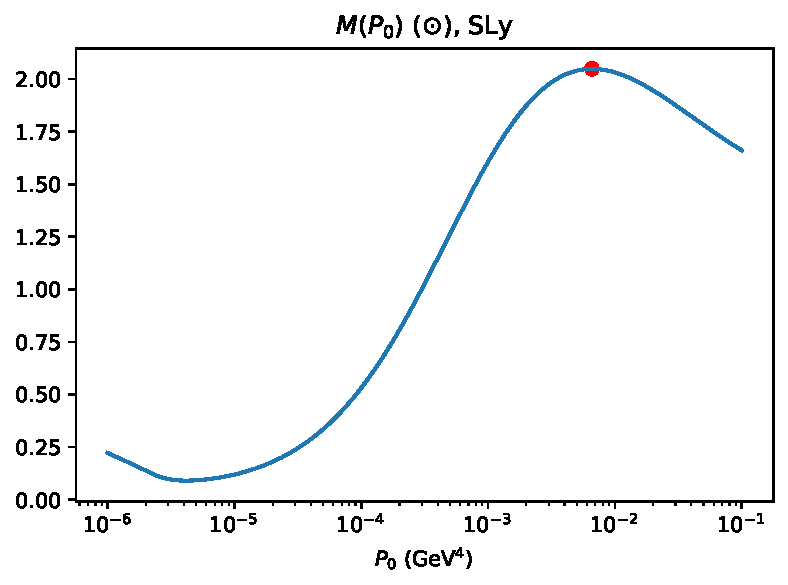
\includegraphics[width = \textwidth]{p0_analysis,SLy.pdf}
            \end{subfigure}
            \caption[]{Example curves for EoS ``SLy.'' $\SI{1}{\odot} = \SI{1.989e+30}{kg}$ (solar mass)}
        \end{figure}
    \end{frame}

    \begin{frame}{Critical Values of $P$, $R$, and $M$}
        \vspace{-10pt}
        \begin{figure}[h!]
            \centering
            \begin{subfigure}{.5\textwidth}
                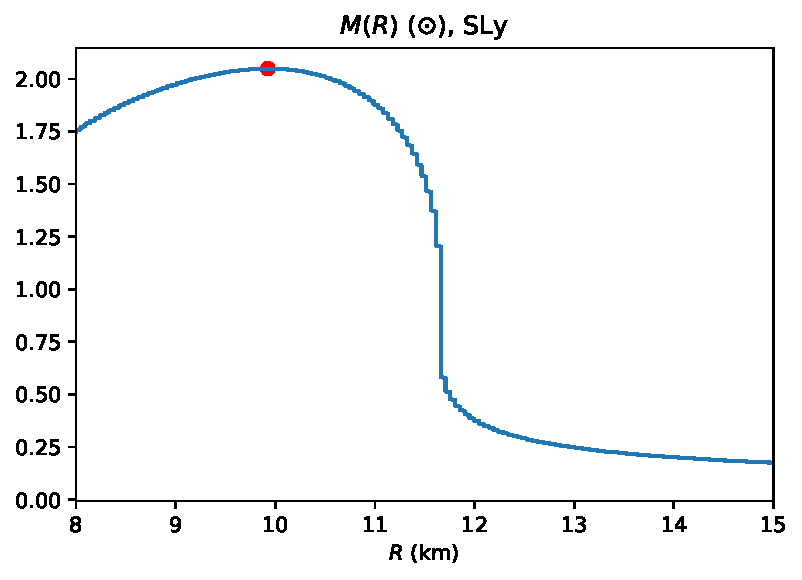
\includegraphics[width = \textwidth]{r_analysis,SLy.pdf}
            \end{subfigure}%
            \begin{subfigure}{.5\textwidth}
                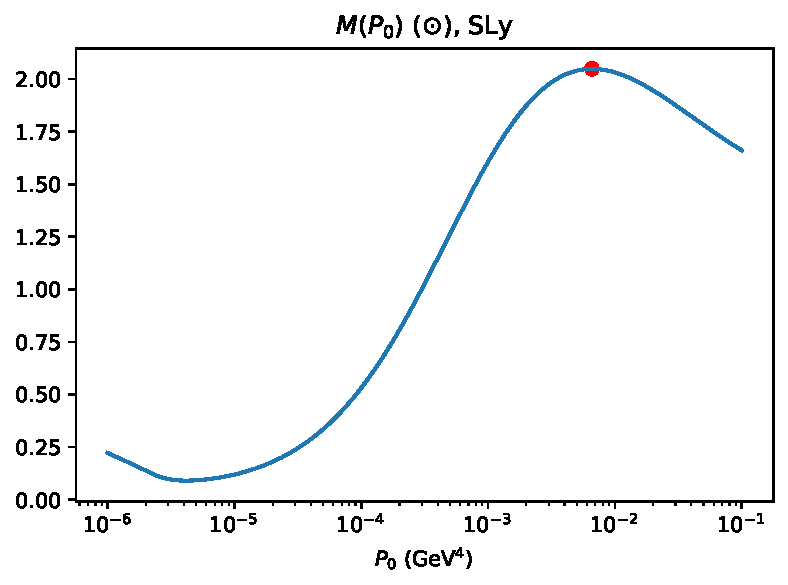
\includegraphics[width = \textwidth]{p0_analysis,SLy.pdf}
            \end{subfigure}
        \end{figure} \pause
        Three important values: \pause \textit{critical pressure, critical mass,} and \textit{critical radius}. \pause 
        \begin{itemize}
            \item Determined by ``peaks'' of graph\pause ; calculated using an optimization routine \pause
            \item Maximum mass and radius predicted by EoS \pause
            \item Largest ``stable'' pressure \pause
            \item SLy: $M_\text{max} = \SI{2.05}{\odot}$, $R_\text{max} = \SI{9.93}{km}$, and $P_\text{crit} = \SI{6.59e-3}{GeV^4}$.
        \end{itemize}

    \end{frame}

    \begin{frame}{Predictions of Other Equations of State}
        \pause
        There are other realistic, analytical fit EoSs of a similar form SLy given in \autocite{SLy_2004,BSk_2013}: \pause FPS, BSk19, BSk20, BSk21 \pause
        \vspace{-10pt}
        \begin{figure}[h!]
            \centering
            \begin{subfigure}{.5\textwidth}
                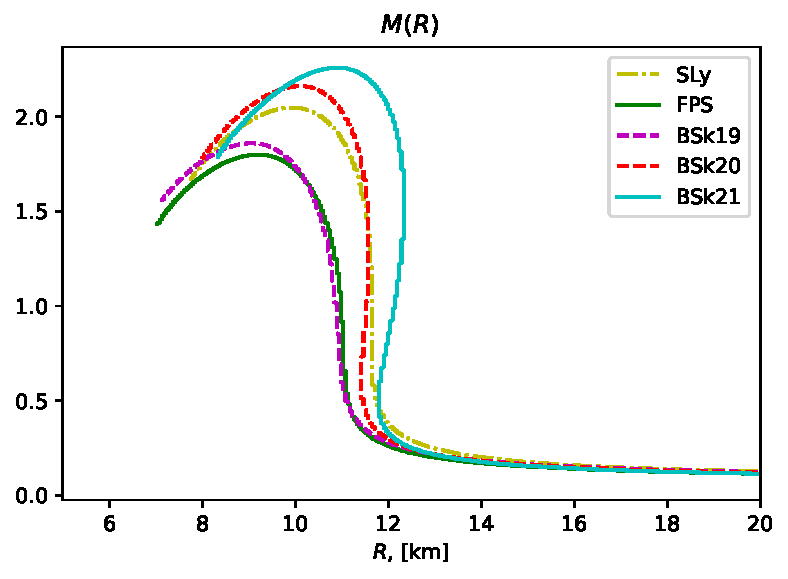
\includegraphics[width = \textwidth]{r_analysis,all.pdf}
            \end{subfigure}%
            \begin{subfigure}{.5\textwidth}
                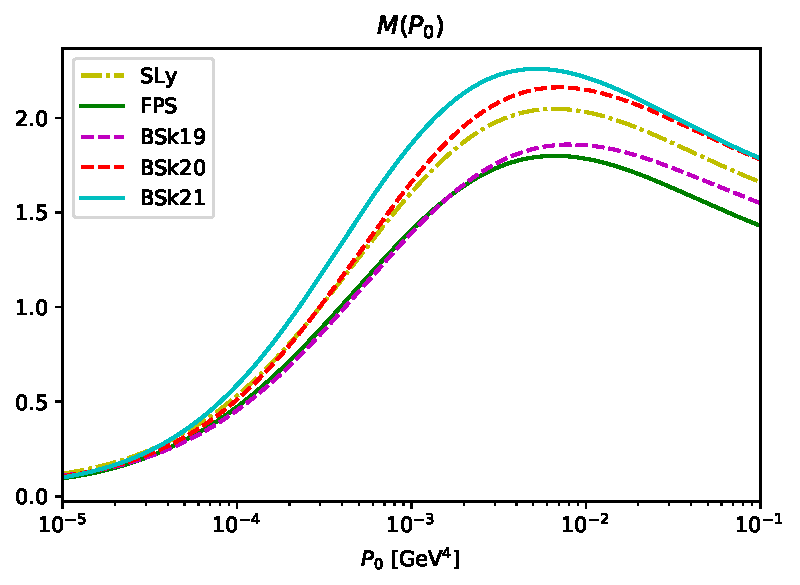
\includegraphics[width = \textwidth]{p0_analysis,all.pdf} 
            \end{subfigure}
            \caption[]{$M(R)$ and $M(P_0)$ for SLy family EoSs. $M$ in \SI{}{\odot}.}
        \end{figure} \pause
        \vspace{-10pt}
        Critical values of the extreme EoSs: \pause
        \begin{itemize}
            \item FPS: $R_\text{max} = \SI{9.20}{km}$, $M_\text{max} = \SI{1.80}{\odot}$, $P_\text{crit} = \SI{6.67e-3}{GeV^4}.$
            \item BSk21: $R_\text{max} = \SI{10.9}{km}$, $M_\text{max} = \SI{2.26}{\odot}$, $P_\text{crit} = \SI{5.17e-3}{GeV^4}.$
        \end{itemize}

    \end{frame}

    \section{Temporal Simulations of Neutron Stars}

    \begin{frame}{Temporal Simulations of Neutron Stars: Background}
        \begin{itemize}
            \pause
            \item Neutron star as a spherically symmetric hydrodynamical system \pause
            \item Three \textit{primitive} variables: pressure $P$, energy density $\epsilon$, and velocity $v$ \pause
            \item $\epsilon$ and $P$ related by an EoS \pause
            \item Define \textit{conservative} variables $\Pi, \Phi$ in terms of primitive variables
            \[\Pi = \frac{\epsilon + P}{1-v} - P, \quad \Phi = \frac{\epsilon + P}{1+v} - P.\] \pause
            \vspace{-15pt}
            \item $\Pi, \Phi$ obey a conservation equation
            \[\p_t \vec{u} = -\frac{1}{r^2}\p_r\pqty{r^2\frac{\alpha}{a}\vec{f}^{(1)}} - \p_r\qty(\frac{\alpha}{a}\vec{f}^{(2)})+\vec{s}, \quad \vec{u} = \mqty[\Pi\\\Phi],\]
            where $a,\alpha$ are the \textit{gravity} variables. \pause
            \item $\vec{f}^{(1)} = \vec{f}^{(1)} (\vec{u}, v),~~ \vec{f}^{(2)} = \vec{f}^{(2)}(P),~~ \vec{s} = \vec{s}~(\vec{u},P,\epsilon,v,a,\alpha)$. \pause
            \item Separate evolution equations for $a,\alpha$
        \end{itemize}
    \end{frame}


    \begin{frame}{Temporal Simulations of Neutron Stars: Background}
        \pause
        \begin{itemize}
        \item Evolve a set of discrete spatial gridpoints $\to$ advanced numerical techniques \pause
        \begin{itemize}
            \item Finite differencing (for spatial derivatives) and the method of lines \pause
            \item High-resolution shock-capturing methods \pause
            \item Evolve through time using numerical integration (Runge-Kutta 3, Modified Euler's Method) \pause
        \end{itemize}
        \item Use EoSs that are analytical fits for numerical stability and root-finding abilities \begin{itemize} \pause
            \item Determine $P,\epsilon,v$ numerically from $\Pi, \Phi$\pause ; need to be able to differentiate (e.g. Newton-Raphson Method) \pause
            \item Extensive studies of realistic, analytical EoSs from \autocite{SLy_2004,BSk_2013}; SLy family
        \end{itemize}
        \end{itemize}
    \end{frame}

    \begin{frame}{Temporal Simulations of Neutron Stars}
        \pause
        \begin{itemize}
            \item Use static solutions as initial data for temporal simulation \pause
            \begin{itemize}
                \item Above \textit{critical pressure}: \pause unstable; below: stable \pause
            \end{itemize}
            \item Stable solutions exhibit \textit{radial oscillations} \begin{itemize} \pause
                \item Evolve out to large $t$ and perform a Fourier transform \pause
            \end{itemize}
        \end{itemize}
            \vspace{-10pt}
        \begin{figure}[h!]
            \centering
            \begin{subfigure}{.5\textwidth}
                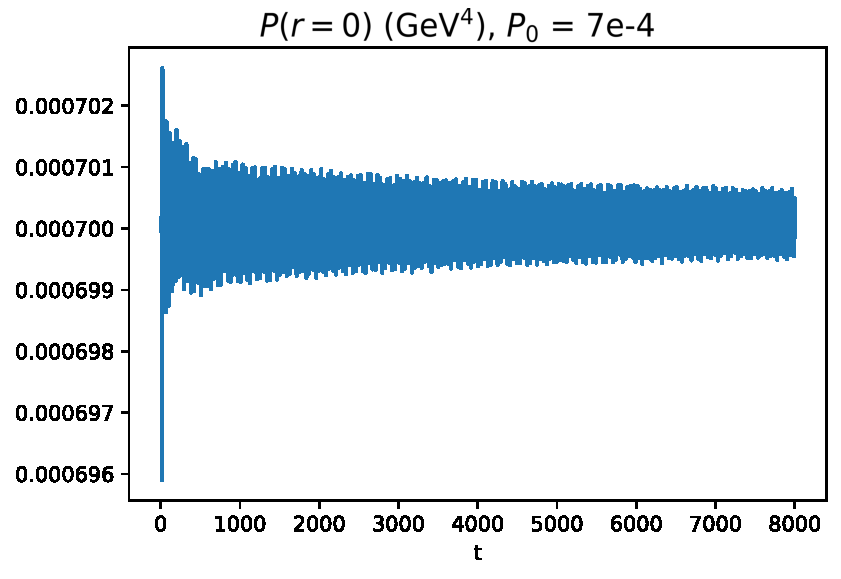
\includegraphics[width = \textwidth]{13-P,ringdown.pdf}
            \end{subfigure}%
            \begin{subfigure}{.5\textwidth}
                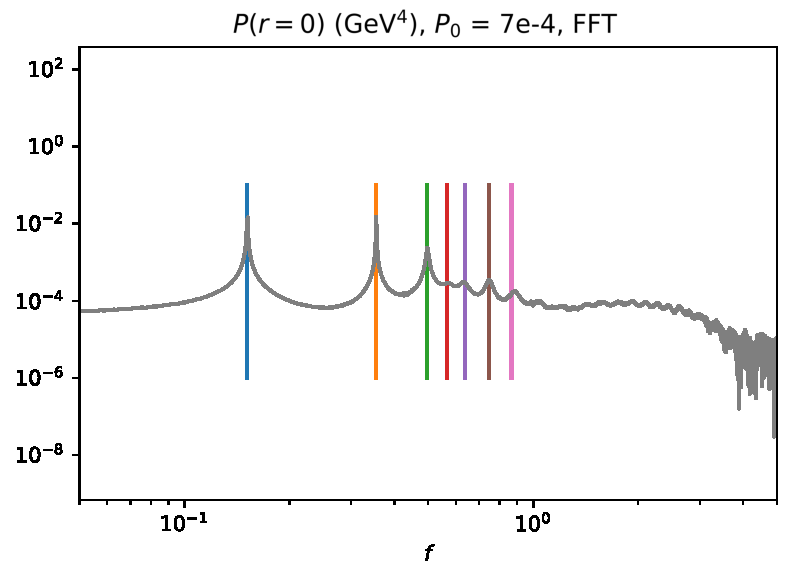
\includegraphics[width = \textwidth]{13-P,ringdown,fft.pdf}
            \end{subfigure}
            \vspace{-10pt}
            \caption[]{Plots of $P(r=0)$ for EoS ``SLy'' and initial $P_0 = \SI{7e-4}{GeV^4}$. Colored lines on FFT plot represent predicted frequencies.}
        \end{figure}
        \vspace{-15pt}
        \begin{itemize} \pause
        \item Radial oscillations differ by EoS; \pause they could soon be measurable!
        \end{itemize}

        % talk about temporal simulation 
        % static solutions as "initial data" for temporal simulation
        % use of analytical fits for equations of state
        % SLy and other realistic equations of state       
    \end{frame}

    % \begin{frame}{Application: Temporal Simulations of Neutron Stars}
    %     % radial oscillations over time; fourier transform
    %     % possible measurement in near future; another observable property
    %     % vary with equation of state; more insight into which EoS may be "correct"
    % \end{frame}

    \begin{frame}{Simulations of Neutron Stars: Nearing Publication}
        ``Dynamical evolution of fermion-boson stars with realistic equations of state'' under Prof. Ben Kain, College of the Holy Cross \pause
        \begin{itemize}
            \item Simulate presence of dark matter as a boson; superimpose a complex scalar field \pause
            \item First temporal simulations of these ``mixed'' stars using \textit{realistic} equations of state; \pause hope is to see how dark matter could affect observable properties of neutron stars \pause
            \item Interesting finding: there is a range of unstable static solutions that \textit{migrate} to stable solutions
        \end{itemize}
    \end{frame}

    \section{Derivation and Computation of an Equation of State}

    \begin{frame}{Computing an EoS: Quantum Hadrodynamics}
        \pause
        A theory of the quantum mechanical, interparticle interactions within a neutron star. \pause
        \begin{itemize}
            \item Formulation of nuclear interactions between \textit{baryons} by the exchange of \textit{mesons} \pause \begin{itemize}
                \item \textit{baryons} are particles containing three quarks (e.g. protons, neutrons) \pause
                \item \textit{mesons} are quark/anti-quark pairs\pause
            \end{itemize}
            \item Requires experimental input for constraint; \pause implemented using \textit{coupling constants} \pause \begin{itemize}
                \item Models the strength of the interactions between particles \pause
                \item Multiple \textit{parameter sets} have been developed by fitting observed nuclear properties of nuclear matter \pause
            \end{itemize}
            \item Considered quite complicated to solve\pause ; we introduce some simplifications in the QHD-I model
        \end{itemize}
    \end{frame}

    % \begin{frame}{Quantum Hadrodynamics}
    %     \pause A theory of the interactions between the subatomic particles in the core of a neutron star
    %     \pause
    %     \begin{itemize}
    %         \item The protons and neutrons influence one another (e.g. apply forces); \pause mediated by exchanging a particle \pause (called a \textit{meson}) \pause
    %         \item Describe these interactions mathematically; \pause the Lagrangian $\Lag$ \pause
    %     \end{itemize}
    %     Model requires input from actual experiments \pause
    %     \begin{itemize}
    %         \item Extreme conditions in core of a neutron star are not reproducible \pause (e.g. pressures are too high, etc.) \pause
    %     \end{itemize}
    %     Equations of Quantum Hadrodynamics are considered very difficult to solve; \pause introduce simplifications in the QHD-I model
    % \end{frame}

    \begin{frame}{Quantum Hadrodynamics I (QHD-I)}
        We form the Lagrange Density for QHD-I: \pause
        \begin{align*}
            \Lag & = \bar{\psi} \bqty{\gamma_\mu(i\p^\mu -g_v V^\mu) - (M-g_\phi\phi)} \psi \nonumber\\
            & \quad + \frac{1}{2} \pqty{\p_\mu \phi \p^\mu \phi - m_\phi^2 \phi^2} - \frac{1}{4} V_{\mu\nu}V^{\mu\nu} + \frac{1}{2} m_v^2 V_\mu V^\mu,
        \end{align*}
        where $V_{\mu\nu}\Def\p_\mu V_\nu - \p_\nu V_\mu$, $\p_\mu \Def \pdv*{x^\mu}.$ The fields:
        \begin{itemize}
            \item Baryon field (protons and neutrons) $\psi(x^\mu)$, with mass $M$ 
            \item Scalar meson field: $\phi(x^\mu)$, with mass $m_\phi$ 
            \item Vector meson field: $V^\mu(x^\mu)$, with mass $m_v$
            \item Experimental coupling constants: $g_v$ and $g_\phi$ \pause
        \end{itemize}
        From $\Lag$, we can determine $\epsilon$ and $P$, the EoS we desire.
    \end{frame}

    \begin{frame}{QHD-I: Derivation of Equations of Motion}
        \begin{align*}
            \Lag & = \bar{\psi} \bqty{\gamma_\mu(i\p^\mu -g_v V^\mu) - (M-g_\phi\phi)} \psi \nonumber\\
            & \quad + \frac{1}{2} \pqty{\p_\mu \phi \p^\mu \phi - m_\phi^2 \phi^2} - \frac{1}{4} V_{\mu\nu}V^{\mu\nu} + \frac{1}{2} m_v^2 V_\mu V^\mu,
        \end{align*}\pause
        Applying the Euler-Lagrange equations for $\Lag$ over a classical field
        \[\p_\nu\qty(\pdv{\Lag}{(\p_\nu \varphi_\alpha)}) - \pdv{\Lag}{\varphi_\alpha} = 0,\]
        for $\varphi_\alpha \in \Bqty{\phi, V^\mu, \psi}$, \pause we obtain the equations of motion:
        \begin{align*}
            &\p_\nu \p^\nu \phi + m_s^2\phi = g_s\bar{\psi}\psi,\\
            &\p_\mu V^{\mu\nu} + m_\omega^2 V^\nu = g_v \bar\psi \gamma^\nu \psi,\\
            &\bqty{\gamma_\mu(i\p^\mu -g_v V^\mu) - (M-g_s\phi)} \psi = 0,\\
        \end{align*}
    \end{frame}

    \begin{frame}{QHD-I: RMF Simplifications}
        We introduce the \textit{Relativistic Mean Field} (RMF) simplifications. \pause We treat the interactions (exchange of mesons) as their average values: \pause
        \[\phi \to \expval{\phi} = \phi_0, \quad V_\mu \to \expval{V_\mu} = V_0, \quad \bar\psi\psi \to \expval{\bar\psi\psi}, \quad \bar\psi\gamma^\mu\psi \to \expval{\bar\psi \gamma^0\psi},\]
        where $\phi_0$ and $V_0$ are constants. \pause This allows us to simplify $\Lag$ considerably: \pause
        \begin{align*}
            \Lag_\text{RMF} = \bar\psi \bqty{i\gamma_\mu\p^\mu - g_v \gamma_0 V_0 - (M-g_s\phi_0)} \psi - \frac{1}{2} m_s^2 \phi_0^2 + \frac{1}{2} m_\omega^2 V_0^2,
        \end{align*} \pause
        Applying the same simplifications to the equations of motions gives:
        \begin{align*}
            & m_s^2 \phi_0^2 = g_s\expval{\bar\psi\psi}\\
            & m_\omega^2 V_0 = g_v\expval{\bar\psi\gamma^0\psi}\\
            & \bqty{i\gamma_\mu\p^\mu - g_v\gamma_0 V_0 - (M - g_s\phi_0)}\psi = 0\\
        \end{align*}

        % Determining $\phi_0$, $V_0$, $\epsilon$, and $P$: \pause $\quad\varphi_\alpha \in \Bqty{\phi_0, V_0, \psi}$
        % \[\p_\nu\qty(\pdv{\Lag}{(\p_\nu \varphi_\alpha)}) - \pdv{\Lag}{\varphi_\alpha} = 0, \quad
        % T^{\mu\nu} = \pdv{\Lag}{(\p_\mu \varphi_\alpha)}\p^\nu \varphi_\alpha - \Lag \eta^{\mu\nu}.\] \pause
        % $$\epsilon = \expval{T^{00}}, \quad P = \expval{T^{ii}}$$
    \end{frame}

    \begin{frame}{QHD-I: Solving for $\epsilon$ and $P$}
        \pause
        We can now solve for $\epsilon$ and $P$. \pause From \autocite{diener_2008}, we have
        \[\epsilon = \expval{T^{00}}, \quad P = \frac{1}{3}\expval{T^{ii}},\]
        where $T^{\mu\nu}$ is the energy momentum tensor, given by
        \vspace{-5pt}
        \begin{align*}
            T^{\mu\nu} = \pdv{\Lag}{(\p_\mu \varphi_\alpha)}\p^\nu \varphi_\alpha - \Lag \eta^{\mu\nu}.
        \end{align*} \pause
        \vspace{-5pt}
        Using $\Lag_\text{RMF}$, we obtain
        \vspace{-5pt}
        \begin{align*}
            T^{\mu\nu}_\text{RMF} & =i\bar\psi\gamma^\mu \p^\nu \psi - \eta^{\mu\nu} \pqty{- \frac{1}{2} m_s^2 \phi_0^2 + \frac{1}{2} m_\omega^2 V_0^2}.
        \end{align*} \pause
        \vspace{-5pt}
        This gives
        \vspace{-15pt}
        \begin{align*}
            \epsilon & = \expval{i\bar\psi\gamma^0 \p^0 \psi} + \frac{1}{2} m_s^2 \phi_0^2 - \frac{1}{2} m_\omega^2 V_0^2,\\
            P & = \expval{i\bar\psi\gamma^i \p^i \psi}  - \frac{1}{2} m_s^2 \phi_0^2 + \frac{1}{2} m_\omega^2 V_0^2.
        \end{align*} \pause
        The above expectation values are non-trivial and are derived in \autocite{diener_2008}.
    \end{frame}

    \begin{frame}{QHD-I: Resulting Equations}
        \pause
        After calculation the expectation values, we obtain the following equations: \pause
        \begin{align*}
            \phi_0 &= \frac{g_\phi}{m_\phi^2} \frac{1}{\pi^2} \int_0^{k_f} \dd{k} \frac{(M-g_\phi \phi_0) k^2 }{\sqrt{k^2 + (M-g_\phi \phi_0)}},  \\
            V_0 &= \frac{g_v}{m_v^2} \frac{k_f^3}{3\pi^2}, \\
            \epsilon & = \frac{1}{2} m_\phi^2 \phi_0^2 + \frac{1}{2} m_v^2 V_0^2 + \frac{1}{\pi^2} \int_0^{k_f} \dd{k} k^2 \sqrt{k^2 + m^{*2}},\\
            P & = -\frac{1}{2} m_\phi^2 \phi_0^2 + \frac{1}{2} m_v^2 V_0^2 + \frac{1}{3} \pqty{\frac{1}{\pi^2} \int_0^{k_f} \dd{k}\frac{k^4}{\sqrt{k^2 + m^{*2}}}}.
        \end{align*}
        where $m^* = (M-g_\phi \phi)$, the \textit{reduced mass}. \pause $k_f$, the Fermi wavenumber, is a free parameter. 
    \end{frame}

    \begin{frame}{Resulting Equations}
        \pause Goal: \pause create a list of values that show us $\epsilon(P)$; \pause each value of $k_f$ gives us a different $\epsilon$ and $P$. \pause

        \medskip
        To produce the EoS: \pause (repeat the following) \pause
        \begin{itemize}
            \item Choose a $k_f$ value \pause
            \item calculate $\phi_0$ and $V_0$\pause; use \textit{rootfinding} for $\phi_0$\pause
            \item Using those values, calculate $P$ and $\epsilon$ and store in a table \pause
        \end{itemize}
        We loop through $k_f$ values until we have a large range of $P$ values \[P\in[\SI{e-20}{}, \SI{e-1}{}] (\SI{}{GeV^4}).\]
    \end{frame}

    % \begin{frame}{Producing the Equation of State}

    %     Steps: \pause
    %         \begin{align*}
    %             \phi_0 = f(k_f, \pause \phi_0), \pause \quad
    %             V_0 = \frac{g_v}{m_v^2} \frac{k_f^3}{3\pi^2} 
    %         \end{align*}
    %         \item Using those values, calculate $P$ and $\epsilon$ and store in a table
    %     \end{itemize}
    % \end{frame}
    
    \begin{frame}{$M(R)$ and $M(P_0)$ Curves for QHD-I}
        We use the tabulated values of $P$ and $\epsilon$ to solve the TOV equations: \pause
        \begin{figure}[h!]
            \centering
            \begin{subfigure}{.5\textwidth}
                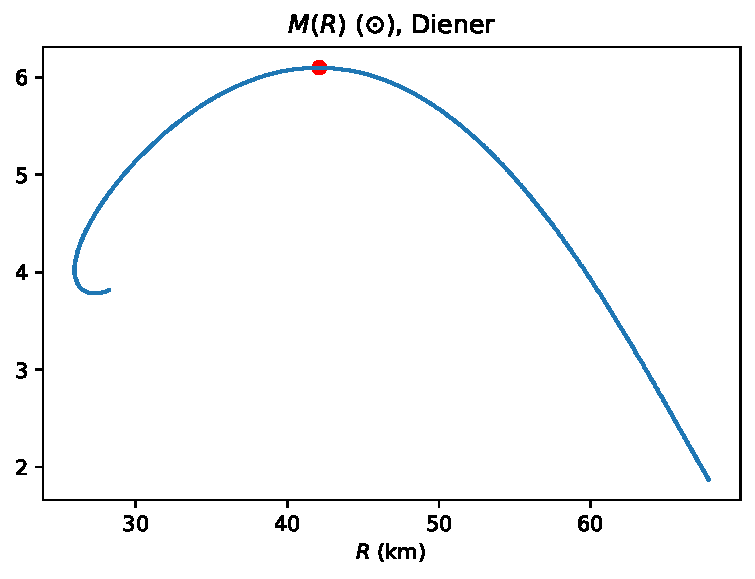
\includegraphics[width = \textwidth]{../paper/images/qhd1/r_analysis.pdf}
            \end{subfigure}%
            \begin{subfigure}{.5\textwidth}
                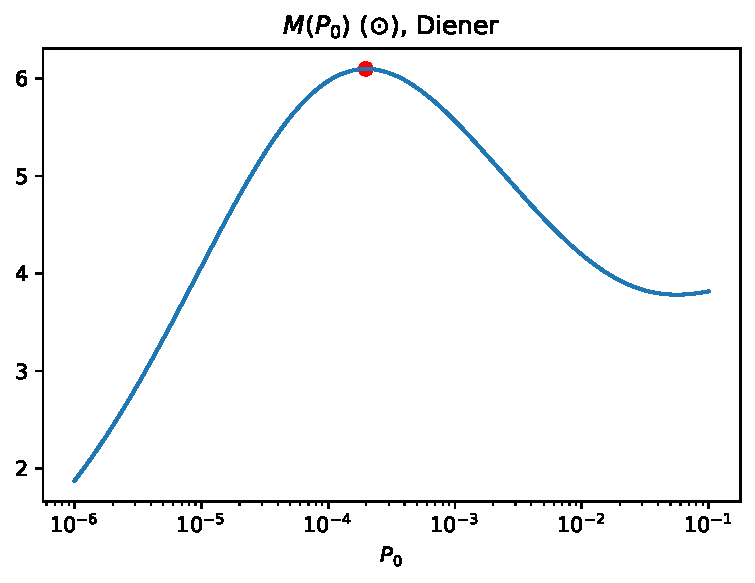
\includegraphics[width = \textwidth]{../paper/images/qhd1/p0_analysis.pdf}
            \end{subfigure}
            \caption[]{$M(R)$ and $M(P_0)$ curves for QHD-I EoS.}
        \end{figure}\pause
        \vspace{-3pt}
        These curves give \[M_\text{max} = \SI{6.1}{\odot}, \quad R_\text{max} = \SI{42.1}{km}, \quad P_\text{crit} = \SI{1.98e-4}{GeV^4}.\]
    \end{frame}

    \begin{frame}{Conclusion}
        \begin{itemize}
            \item An equation of state is a relationship between energy density and pressure within a neutron star \pause
            \item We use the TOV equations to predict the maximum mass and radius that a given EoS will produce \pause
            \item Within a temporal simulation of a neutron star: \pause \begin{itemize}
                \item Static solutions are used as initial data \pause
                \item We can predict radial oscillation frequencies of neutron stars, which could soon be measurable \pause
            \end{itemize}
            \item We use the QHD-I parameter set and RMF simplifications to solve a system of equations and generate an equation of state
        \end{itemize}
    \end{frame}

    \begin{frame}[allowframebreaks]{References}
        \nocite{*}
        \printbibliography
    \end{frame}


\end{document}
